\section{Vorbereitung}

\noindent{\large Arbeitsaufteilung:\par}
\begin{table}[htb]
\centering
\caption{Arbeitsaufteilung in der Gruppe}
\label{Arbeitsaufteilung}
\begin{tabular}{c|ccc}
\toprule
Aufgabe & Lucas & Aleksandra & Timo\\
\midrule
Motivation &  & x & \\
Literaturrecherche &  &  & x\\
Lüfterschaltung & x & x & x\\
Geschwindigkeitsmessanlage & x & x & x\\
Dokumentation & x & x & x\\
Diskussionen & x & x & x\\
Bericht \& Spice & x &  & \\
\bottomrule
\end{tabular}
\end{table}

\noindent{\large Genutzte Materialien:\par}
\begin{table}[htb]
\centering
\caption{Genutzte Materialien}
\label{Materialien}
\begin{tabular}{c|c}
\toprule
Bauteiltyp & Beschreibung\\
\midrule
Launchpad & Tiva C Series, 1x \\
\hline
Heißleiter & 
\vtop{
\hbox{\strut NTCLE100E3 (Vishay):}
\hbox{\strut ~~~~$R_{25} = 10k\Omega$ (Toleranz $\pm 5\%$),}
\hbox{\strut ~~~~$B_{25/85} = 3977K$ (Toleranz $\pm 0.75\%$), 1x}
} \\
\hline
Lichtschranke & 
\vtop{
\hbox{\strut Emitter: V472P}
\hbox{\strut Detektor: S472P}
\hbox{\strut TELEFUNKEN Semiconductors}
} \\
\hline
Transistor & BC547C (STMicroelectronics) \\
\hline
Speicherkondensatoren & diverse (Toleranz $\pm 20\%$) \\
\hline
Kohleschichtwiderstände & diverse (Toleranz $\pm 5\%$) \\
\bottomrule
\end{tabular}
\end{table}

\clearpage
\section{Einleitung}

\subsection{Motivation}


\subsection{Literaturrecherche}


\clearpage
\section{Aufgaben}

\subsection{Lüfterschaltung}

\subsubsection{Materialien \& Methoden}

\begin{figure}[htb]
    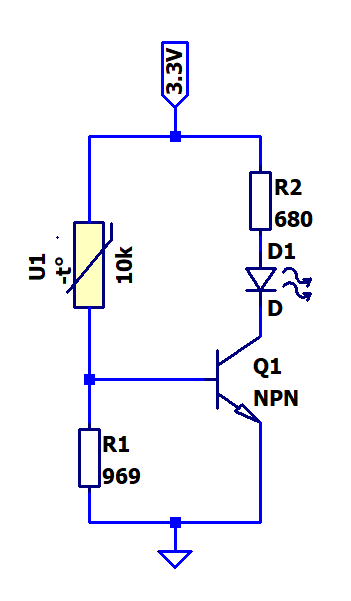
\includegraphics[width=4cm]{./res/Luefter_1_Spice}
    \caption{Aufbau der 1. Lüfterschaltung}
    \label{fig:Lüfterschaltung1}
\end{figure}

\begin{figure}[htb]
    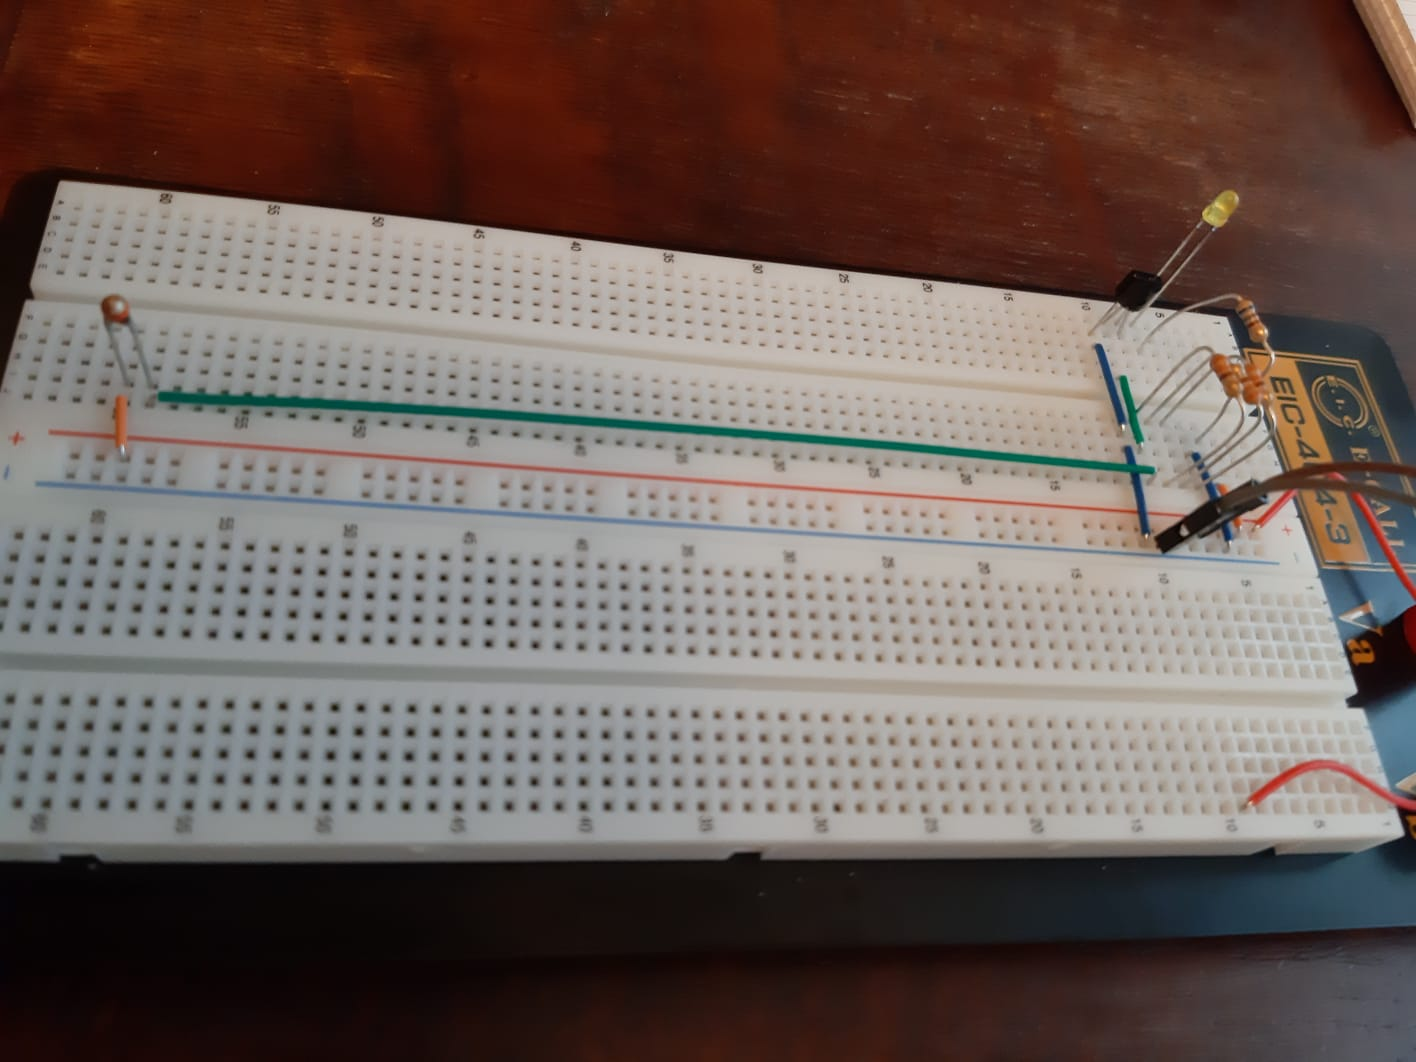
\includegraphics[width=12cm]{./res/Luefter_1_Aufbau}
    \caption{Praktischer Aufbau der 1. Lüfterschaltung}
    \label{fig:Lüfterschaltung1Praktisch}
\end{figure}

\newpage
\noindent
Durch folgende Rechnungen konnten wir auf die Widerstandswerte schließen: \\
\\
Wie in der Aufgabenstellung gefordert, soll die Leistung des NTCs auf $15 mW$ beschränkt sein. Hierfür wird für den vorhandenen Arbeitsbereich ($25^{\circ} C - 100^{\circ} C$) eine Berechnung des Widerstands $R_1$ benötigt. Der Widerstand bildet mit dem variablen Widerstandswert des NTCs den Gesamtwiderstand, von welchem aus die Leistung des NTCs berechnet werden kann. Vor die Basis des Transistors wird ein Widerstand geschalten, für welchen gilt: $R_B >> R_1$. Somit ist der Strom $I_B$ in den Rechnungen vernachlässigbar klein.\\
\\
% http://www.vishay.com/docs/29049/ntcle100.pdf
Widerstand des NTCs bei $25^{\circ} C: 10 k\Omega$; $150^{\circ} C: 182,6 \Omega$ \cite{ntc} \\
\\
Berechnung des minimalen Widerstands $R_1$ zur Einhaltung der Leistungsvorgabe:
\[ R_{ges} = 182.6 \Omega + R_1 \]
\[ I_{ges} = \frac{3.3 V}{R_{ges}} \]
\[ U_{NTC} = 182.6 \Omega \cdot I_{ges} \]
\[ P_{NTC} = 182.6 \Omega \cdot \left(\frac{3.3 V}{R_{ges}}\right)^2 = 15\cdot10^{-3} W \]

\gleichung{
\begin{split}
\frac{182.6 \Omega \cdot (3.3 V)^2}{(182.6 \Omega + R_1)^2} &= 15.10^{-3} W
\\
(182.6 \Omega + R_1)^2 &= \frac{182.6 \Omega \cdot (3.3 V)^2}{15.10^{-3} W}
\\
182.6 \Omega + R_1 &= 3.3 V \cdot \sqrt{\frac{182.6 \Omega}{15.10^{-3} W}}
\\
R_1 &= 3.3 V \cdot \sqrt{\frac{182.6 \Omega}{15.10^{-3} W}} - 182.6 \Omega
\\
R_1 &= 181.5 \Omega
\end{split}
}{}

\noindent
Daraus folgt, dass $R_1 > 181.5 \Omega$ gilt, da ansonsten über den NTC mehr als 15 mW abfallen würden. \\
\\
Da der NTC einen negativen Temperaturkoeffizienten besitzt, steigt sein Widerstand bei sinkender Betriebstemperatur und sinkt analog bei steigender Betriebstemperatur. Daraus folgt ein geringerer Strom für Temperaturen unter $150^{\circ} C$ und damit einhergehend eine geringere Leistung am NTC. Unser Arbeitsbereich beschränkt sich auf 25 - 150 Grad, somit ist diese Folgerung ausreichend für unseren Anwendungsbereich. \\

\newpage

\noindent
Eine gelbe LED besitzt einen Spannungsabfall von $2.2 V$. Deshalb muss über die vor den LEDs geschalteten Widerstände eine Spannung von jeweils $1.1 V$ abfallen. Wählt man einen Widerstand von $680 \Omega$, so beträgt der Strom $1.618 mA$. Dabei fallen über der LED genau $2.2 V$ ab. \cite{diode}

\begin{figure}[htb]
    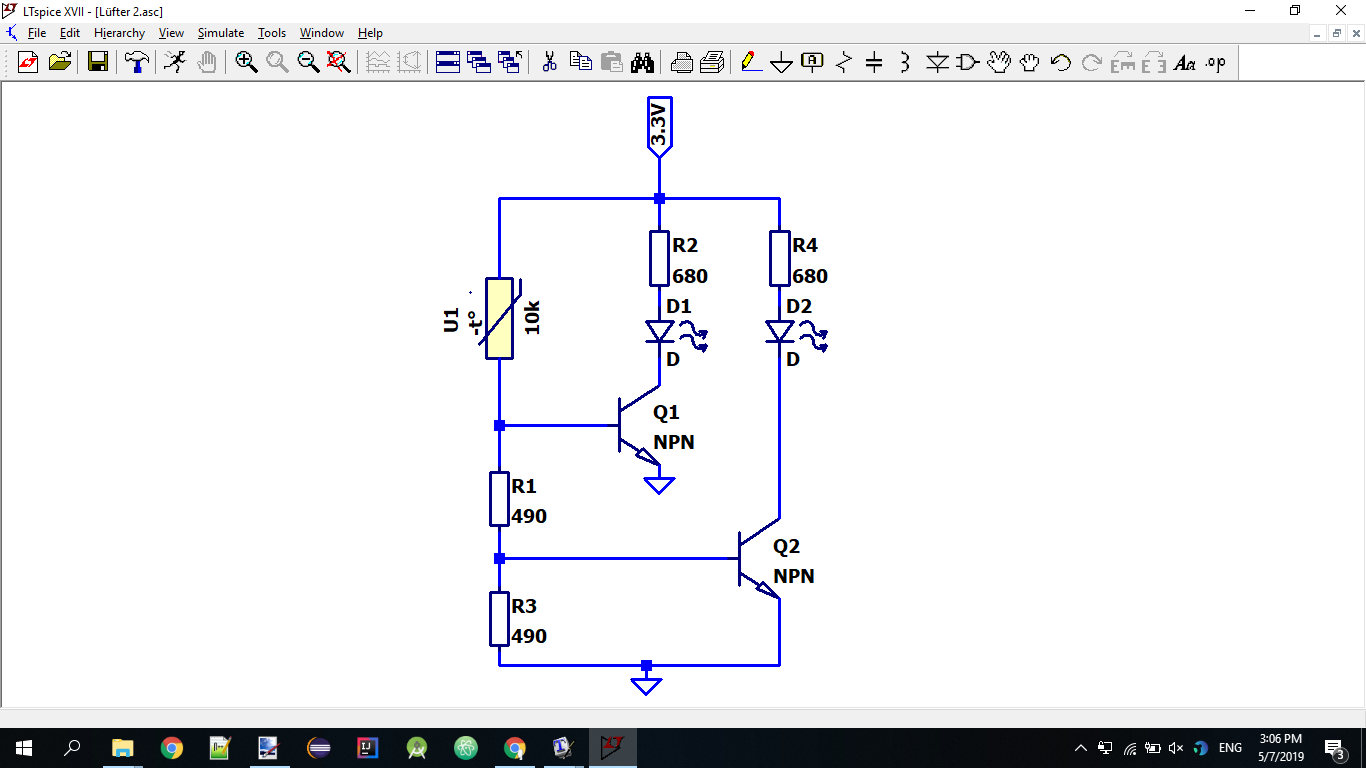
\includegraphics[width=4cm]{./res/Luefter_2_Spice}
    \caption{Aufbau der 2. Lüfterschaltung}
    \label{fig:Lüfterschaltung2}
\end{figure}

\begin{figure}[htb]
    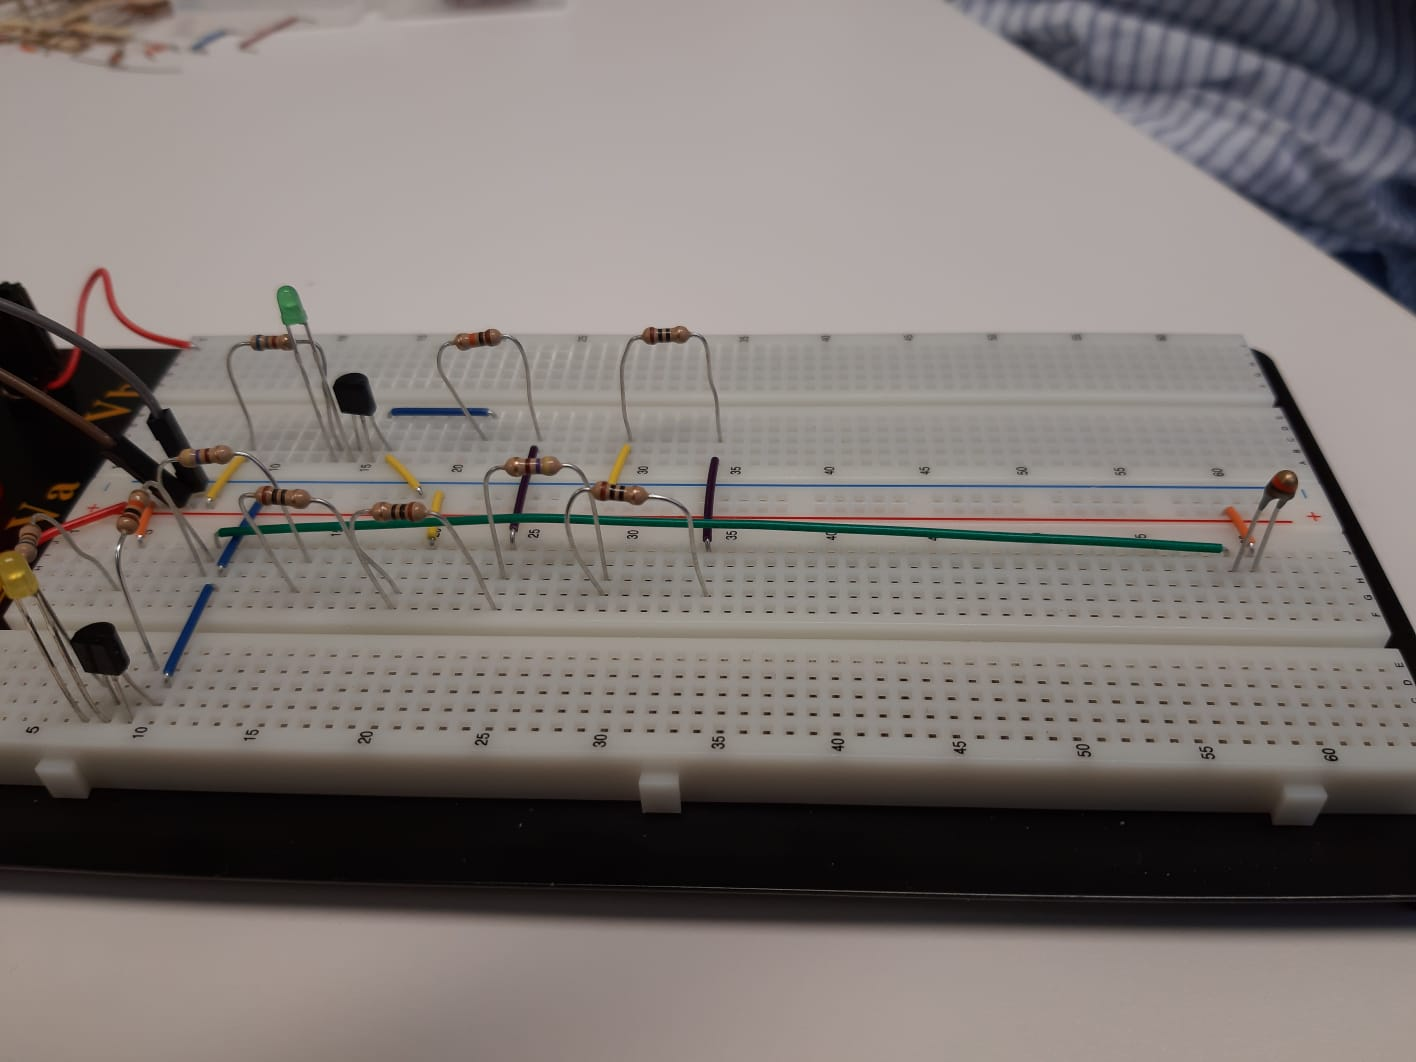
\includegraphics[width=12cm]{./res/Luefter_2_Aufbau}
    \caption{Praktischer Aufbau der 2. Lüfterschaltung}
    \label{fig:Lüfterschaltung2Praktisch}
\end{figure}

\noindent
Notiz: Wir haben den NTC soweit außerhalb positioniert, um Interferenz mit den anderen Bauteilen (z.B. den Transistoren) zu vermeiden. Wir schalten vor der Diode einen Widerstand mit $100 k \Omega$, um eine Verfälschung unserer Rechnung vorzubeugen und für jede Temperatur den zulässigen Diodenstrom einhalten zu können.

\newpage

\subsubsection{Aufgabe 2.1: Rechnung Lüfterschaltung 1}

Laut Aufgabe soll ein Lüfter ab einer Temperatur von $49^{\circ} C$ in Betrieb genommen werden. Der NTC besitzt bei $50^{\circ} C$ einen Widerstandswert von $3605 \Omega$. Um eine Schaltung des Lüfters bei dieser Temperatur zu konzipieren, muss der Widerstand $R_1$ passend gewählt werden. Da die Schaltschwelle bei $49^{\circ} C$ stattfinden soll, nehmen wir als Widerstandswert des NTCs $3600 \Omega$ an.

\[ R_{ges} = 3600 \Omega + R_1 \]
\[ I_{ges} = \frac{U}{R_{ges}} = \frac{3.3 V}{3600 \Omega + R_1} \]

\gleichung{
\begin{split}
U_{R1} = 0.7 V &= R_1 \cdot I_{ges} = R_1 \cdot \frac{3.3 V}{3600 \Omega + R_1}
\\
3.3 V \cdot R_1 &= 2520 V \cdot \Omega + 0.7 V \cdot R_1
\\
2.6 V \cdot R_1 &= 2520 V \cdot \Omega
\\
R_1 &= 969.23 \Omega \geq 181.5 \Omega
\end{split}
}{}

\subsubsection{Aufgabe 2.2: Rechnung Lüfterschaltung 2}

Laut Aufgabe soll ein zweiter Lüfter ab einer Temperatur von $78^{\circ} C$ in Betrieb genommen werden. Der NTC besitzt bei $78^{\circ} C$ einen Widerstandswert von ca. $1330 \Omega$. Um eine Schaltung des Lüfters bei dieser Temperatur zu konzipieren, muss der Widerstand $R_1$ passend gewählt werden. Außerdem besitzt der NTC bei $80^{\circ} C$ einen Widerstandswert von $1256 \Omega$. \cite{ntc}

\[ R_{ges} = 1330 \Omega + R_1 + R_2\]
\[ R_1 = R_2 \]
\[ R_{ges} = 1330 \Omega + 2 \cdot R_1 \]
\[ I_{ges} = \frac{U}{R_{ges}} = \frac{3.3 V}{1330 \Omega + 2 \cdot R_1} \]
\[ U_{1} = 2 \cdot R_1 \cdot I_{ges} = 2 \cdot R_1 \cdot \frac{3.3 V}{1330 \Omega + 2 \cdot R_1} \]

\gleichung{
\begin{split}
U_{R1} = 1.4 V &= \frac{6.6 V \cdot R_1}{1330 \Omega + 2 \cdot R_1}
\\
1.4 V \cdot (1330 \Omega + 2 \cdot R_1) &= 6.6 V \cdot R_1
\\
1862 V \cdot \Omega \cdot 2.8 V \cdot R_1 &= 6.6 V \cdot R_1
\\
R_1 &= 490 \Omega \geq 181.5 \Omega
\end{split}
}{}

\noindent
Überprüfung des Widerstandswertes bei $50^{\circ} C$ Schaltschwelle

\[ R_{ges} = 3605 \Omega + 2 \cdot 490 \Omega = 4585 \Omega \]
\[ I_{ges} = \frac{U}{R_{ges}} = \frac{3.3 V}{4585 \Omega} = 0.72 mA \]
\[ U = R_{ges} \cdot I_{ges} = 4585 \Omega \cdot 0.72 mA = 0.705 V \]

\noindent
Somit ist unser errechneter Widerstand für beide Schaltungsteile verwendbar, da bei $49^{\circ} C$ die Spannung U minimal geringer wäre.

\subsubsection{Diskussion}

Wie in der Aufgabenstellung gefordert, erwärmten wir den NTC, um die Funktionalität der Schaltung zu überprüfen. Dabei benutzten wir abwechselnd ein Feuerzeug (Abstand 10cm) und einen Fön (Abstand 5cm), um unterschiedlich präzise Ergebnisse zu erzielen. Beim praktischen Test funktionierte die Schaltung wie erwartet, denn die erste LED leuchtete ab ca. $50^{\circ} C$. Ab einer weiteren Erhitzung leuchtete auch die zweite LED nach kurzer Zeit. Beim Abkühlen erlosch die zweite LED zuerst, gefolgt von der ersten LED nach einer zeitlichen Verzögerung. Somit wäre unsere Schaltung als Lüfterschaltung praxistauglich.


\newpage
\subsection{Lichtschranke}

\subsubsection{Materialien \& Methoden}

Spannungsverlauf von $U_{Out}$ bei bewegtem Körper:

\begin{figure}[htb]
    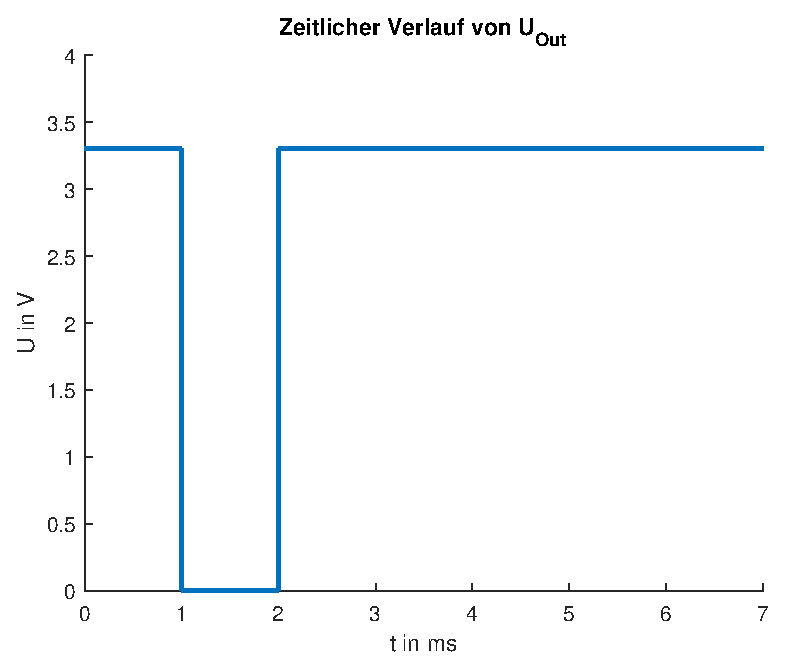
\includegraphics[width=10cm]{./res/Lichtschranke_Spannungsverlauf}
    \caption{Spannungsverlauf von $U_{Out}$}
    \label{fig:SpannungsverlaufUout}
\end{figure}

\begin{figure}[htb]
    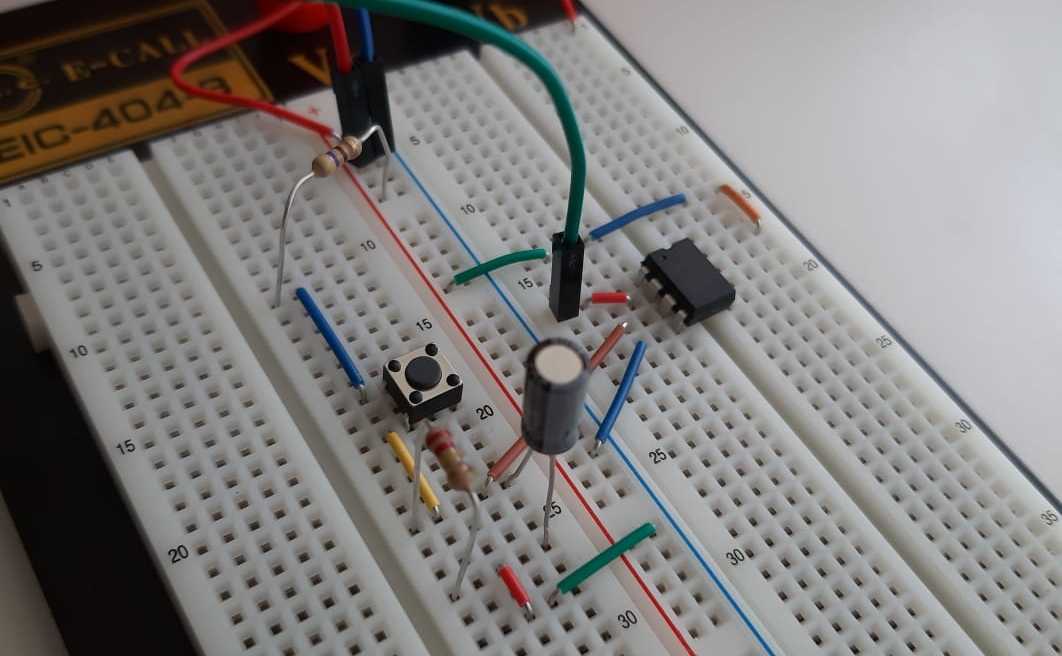
\includegraphics[width=10cm]{./res/Kondensator_Entladung}
    \caption{Schaltung zur Messung der Entladung eines Kondensators}
    \label{fig:KondensatorEntladung}
\end{figure}

\newpage

\begin{figure}[htb]
    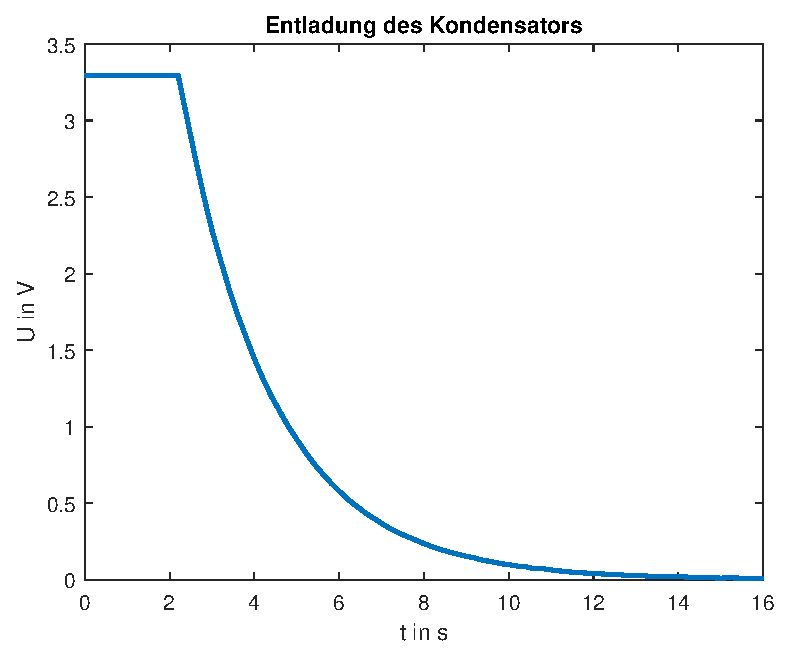
\includegraphics[width=10cm]{./res/Kondensator_Entladung_Messung}
    \caption{Gemessene Entladung des Kondensators}
    \label{fig:KondensatorEntladungMess}
\end{figure}

\begin{figure}[htb]
    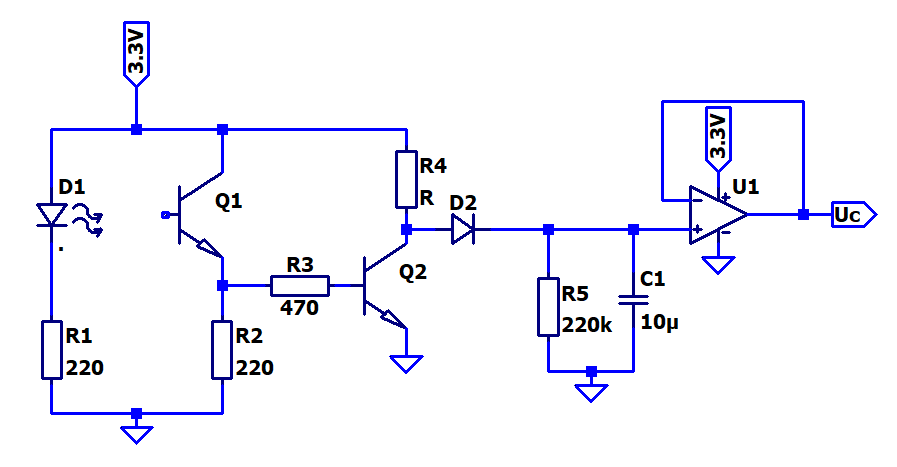
\includegraphics[width=14cm]{./res/Lichtschranke_1_Spice}
    \caption{Schaltung zur Messung der Ladung und Entladung eines Kondensators durch eine Lichtschranke}
    \label{fig:KondensatorLadungLichtschranke}
\end{figure}

\newpage

\begin{figure}[htb]
    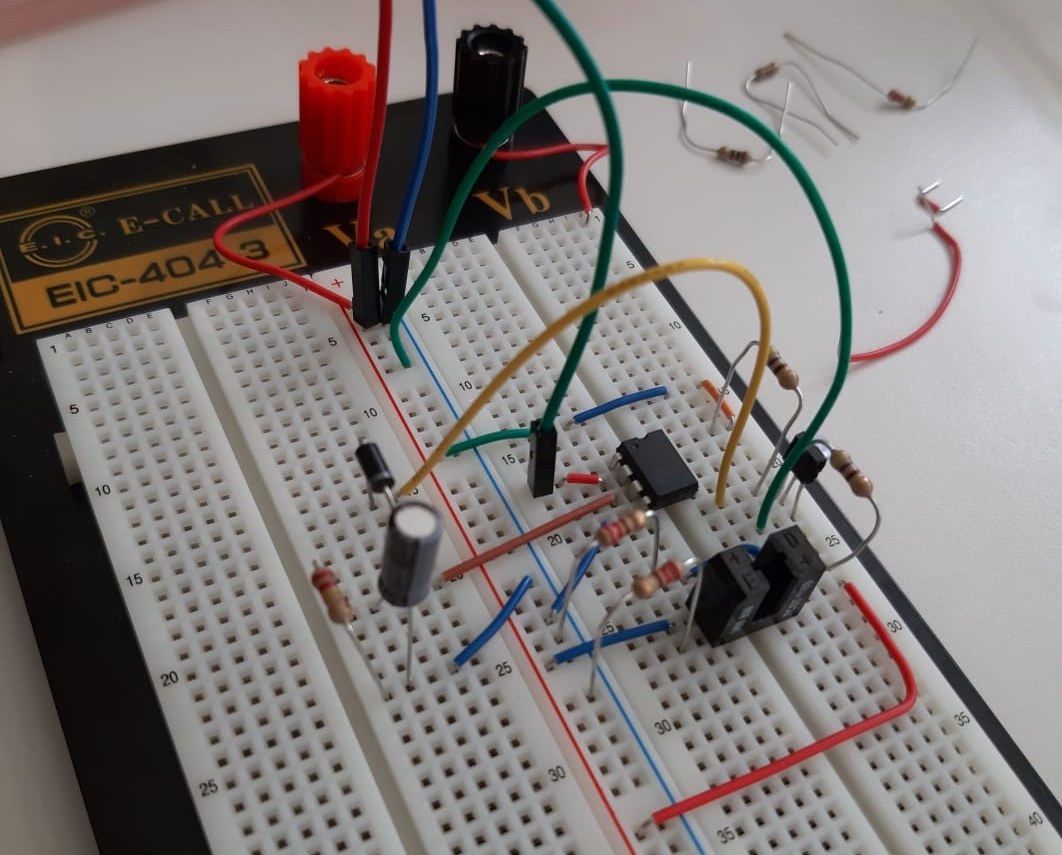
\includegraphics[width=10cm]{./res/Kondensator_Lichtschranke_1}
    \caption{Praktischer Aufbau 1 Lichtschranke}
    \label{fig:KondensatorLadungLichtschrankeAufbau}
\end{figure}

\begin{figure}[htb]
    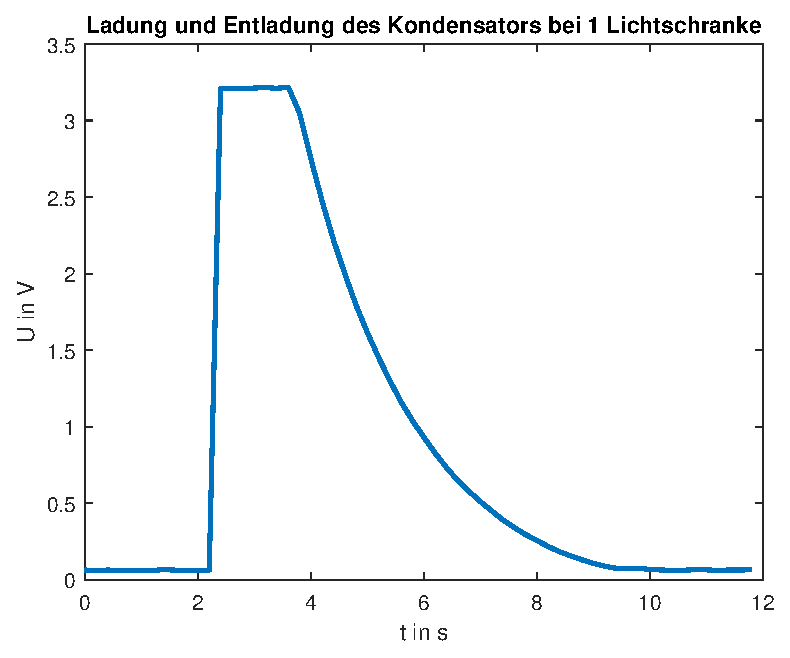
\includegraphics[width=10cm]{./res/Kondensator_1_Lichtschranke_Messung}
    \caption{Gemessene Ladung und Entladung des Kondensators bei 1 Lichtschranke}
    \label{fig:KondensatorLadungEntladungMess}
\end{figure}

\newpage

\begin{figure}[htb]
    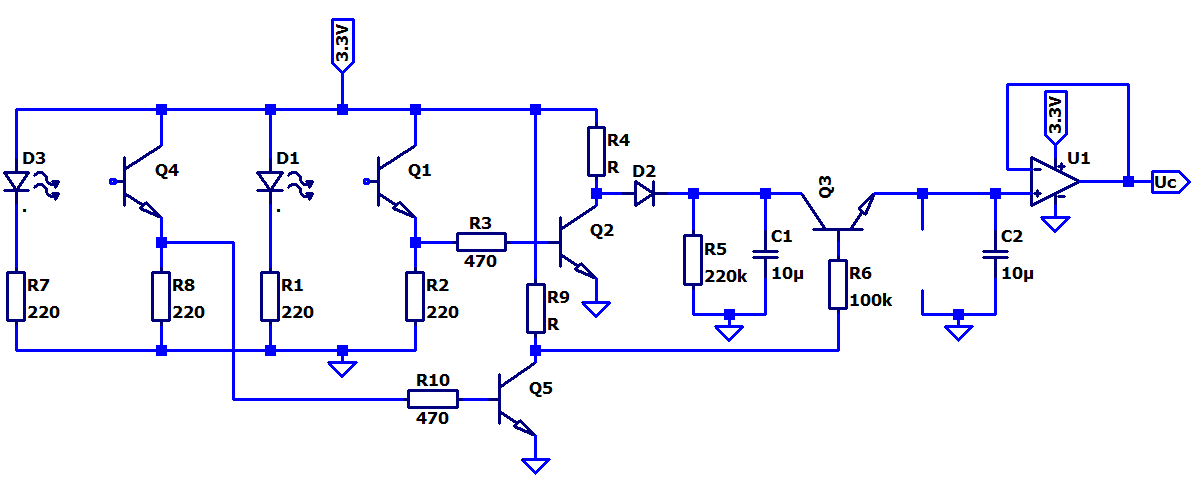
\includegraphics[width=14cm]{./res/Lichtschranke_2_Spice}
    \caption{Schaltung zur Messung der Ladung und Entladung eines Kondensators durch zwei Lichtschranken}
    \label{fig:KondensatorLadungLichtschranke2}
\end{figure}

\begin{figure}[htb]
    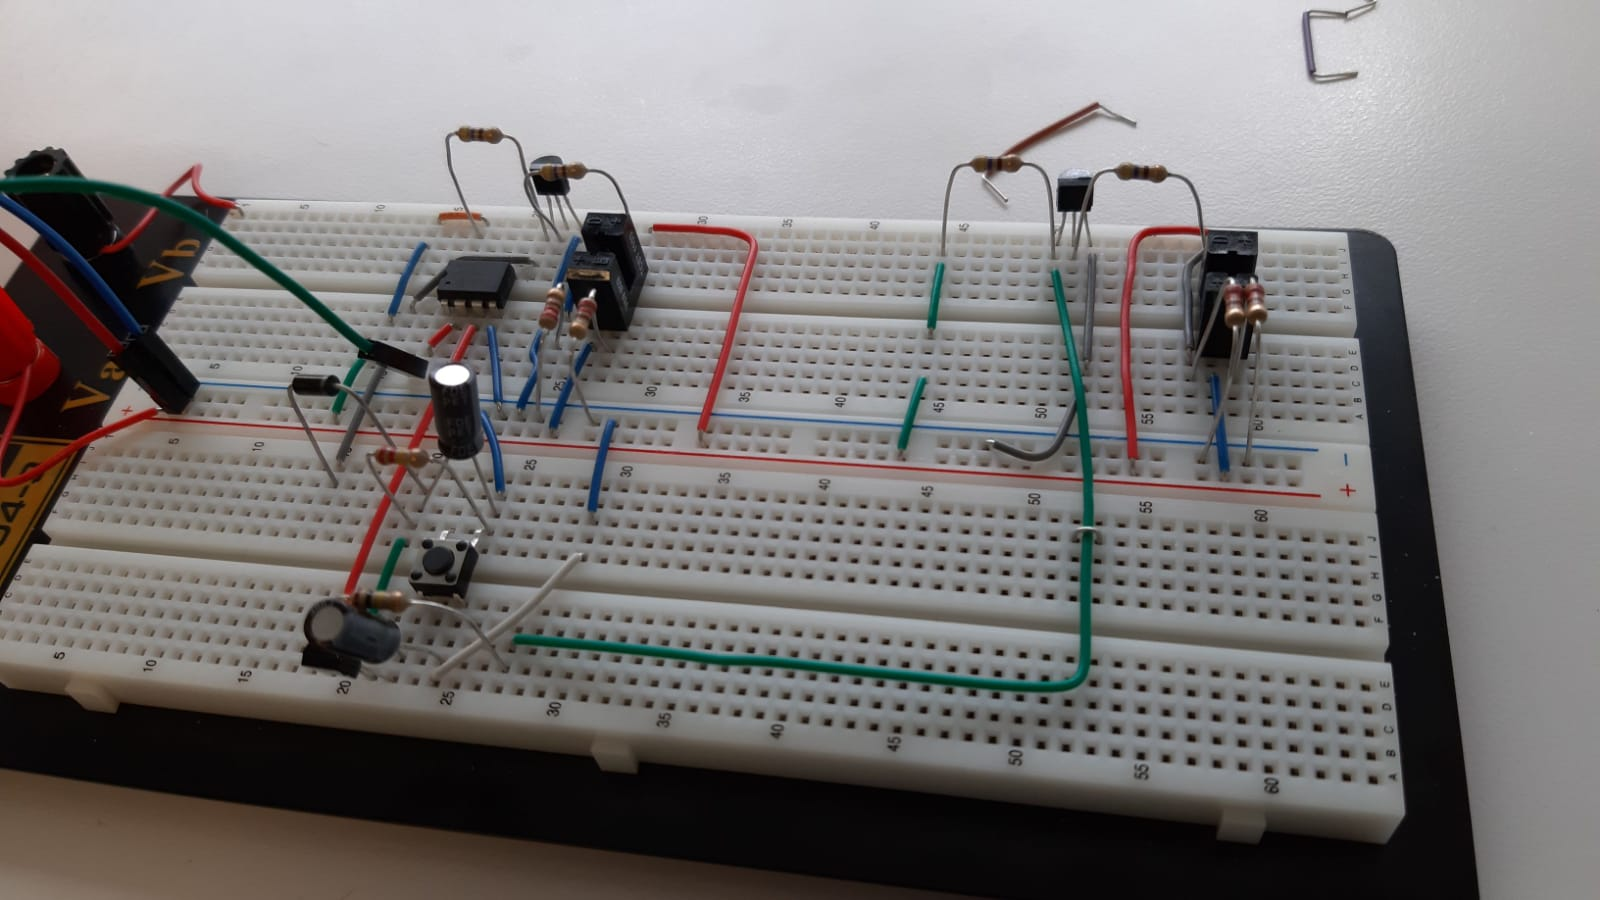
\includegraphics[width=14cm]{./res/Kondensator_Lichtschranke_2}
    \caption{Praktischer Aufbau 2 Lichtschranken}
    \label{fig:KondensatorLadungLichtschrankeAufbau2}
\end{figure}

\newpage
\subsubsection{Entladung Kondensator}

\gleichung{
U_{c}(t)=U_{0} \cdot e^{- \frac{t}{R_{C} \cdot C}}
}{EntladungKondensatorFormel}

\begin{table}[htb]
\centering
\caption{Entladung Kondensator}
\label{KondensatorRechnung}
\begin{tabular}{c|cccccc}
\toprule
t & 0 sec & 1 sec & 2 sec & 3 sec & 4 sec & 5 sec \\
\midrule
$U_{c}(t)$ errechnet & 3.3V & 2.09V & 1.33V & 0.84V & 0.54V & 0.34V \\
$U_{c}(t)$ gemessen & 3.3V & 2.089V & 1.31V & 0.835V & 0.527V & 0.335V \\
\bottomrule
\end{tabular}
\end{table}

\subsubsection{Laden des Kondensators}

Um den Kondensator zu laden, schalten wir zwischen Diode und Transistor einen invertierenden Transistor mit Widerstandsverhältnis = 1, um das gewünschte Schaltverhalten der Lichtschranke zu erzielen.\\
Bei Durchtrennen der Lichtschranke lädt sich der Kondensator über den gewählten $470 \Omega$ Widerstand am Emitter des Invertierers sofort voll auf und entlädt sich, wie im vorherigen Aufgabenteil langsam, über den $220 k \Omega$ Widerstand bei Freilassen der Lichtschranke.\\
Die Diode zwischen Kondensator und Invertierer dient dazu, die Entladung des Kondensators auf den Widerstand mit $220 k \Omega$ zu beschränken.

\subsubsection{Geschwindigkeitsmessanlage}

\begin{figure}[htb]
    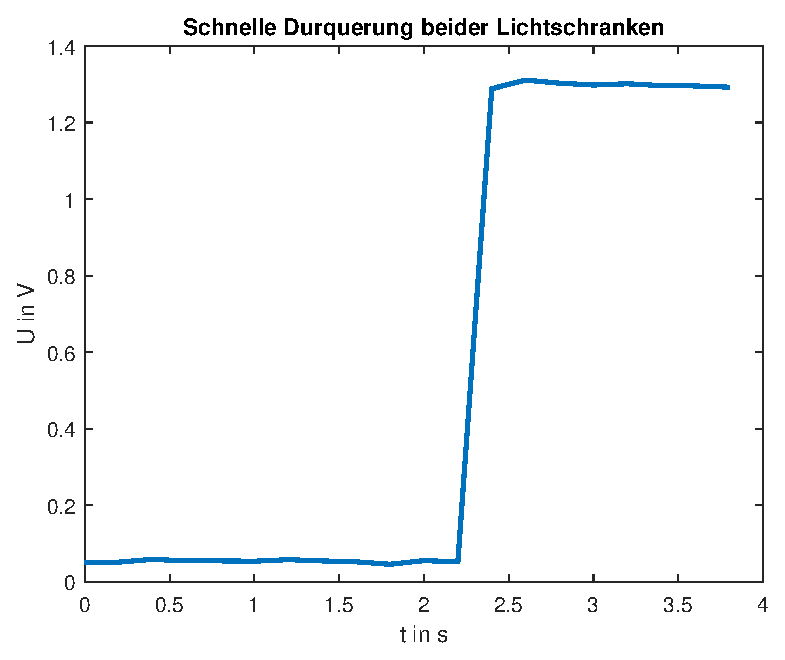
\includegraphics[width=7cm]{./res/Lichtschranke_2_schnell_Messung}
    \caption{Ladung der Kondensatoren bei schneller Durchquerung}
    \label{fig:DurchquerungSchnell}
\end{figure}

\newpage

\begin{figure}[htb]
    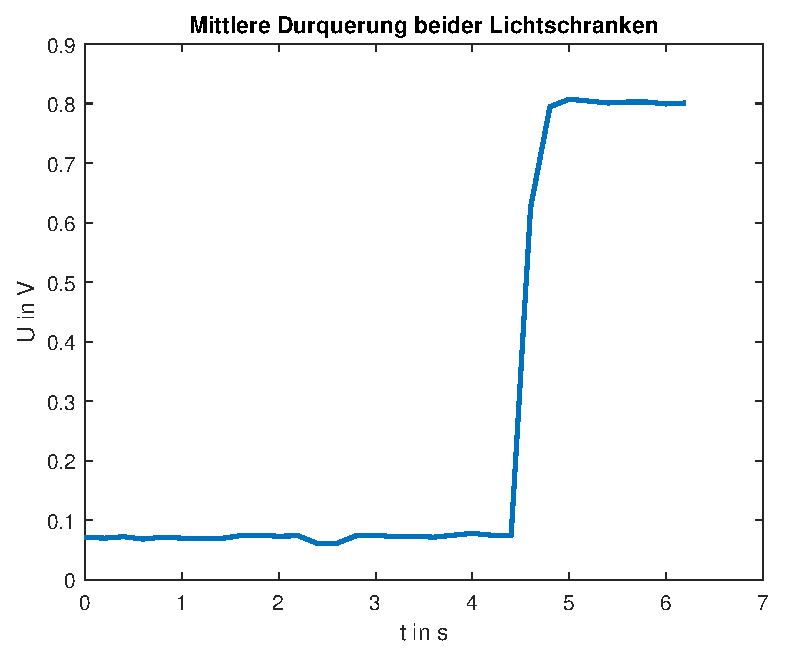
\includegraphics[width=7cm]{./res/Lichtschranke_2_medium_Messung}
    \caption{Ladung der Kondensatoren bei mittlerer Durchquerung}
    \label{fig:DurchquerungMedium}
\end{figure}

\begin{figure}[htb]
    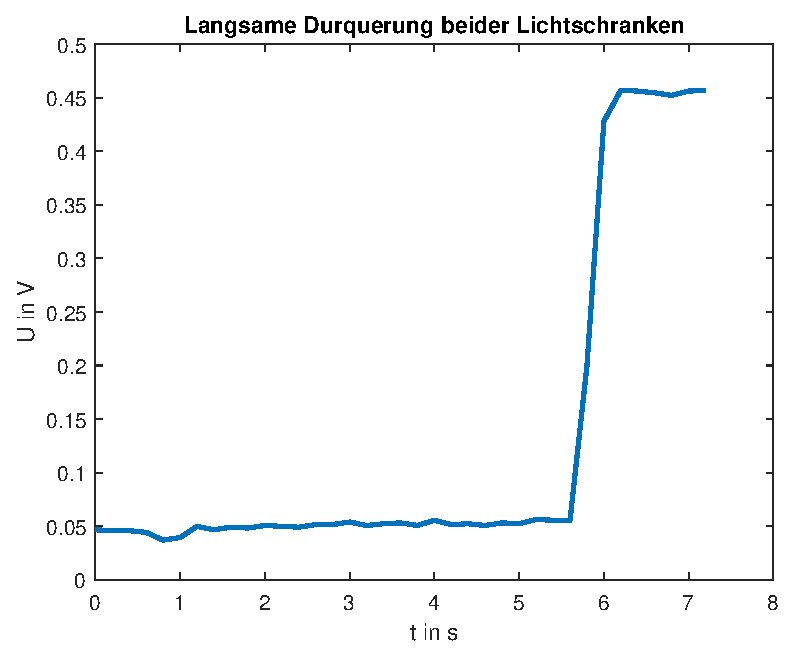
\includegraphics[width=7cm]{./res/Lichtschranke_2_langsam_Messung}
    \caption{Ladung der Kondensatoren bei langsamer Durchquerung}
    \label{fig:DurchquerungLangsam}
\end{figure}

Die Zeit wurde mit der Formel zur Entladung des Kondensators (\ref{EntladungKondensatorFormel}) durch Auflösen nach $t$ berechnet.
\\
\\
Formel zur Berechnung der Geschwindigkeit (konstant ohne Beschleunigung):

\gleichung{
v=\frac{s}{t}=\frac{8 cm}{t}
}{geschw}

\newpage

\begin{table}[htb]
\centering
\caption{2 Lichtschranken Messungen}
\label{Lichtschranken2Messung}
\begin{tabular}{c|cccc}
\toprule
Messung & 1 & 2 & 3 \\
\midrule
Gemessene Spannung & 1.3 V & 0.8V & 0.45V \\
Kondensatorspannung & 2.6V & 1.6V & 0.9V \\
Resultierende Zeit & 0.52 sec & 1.59 sec & 2.86 sec \\
Resultierende Geschwindigkeit & 15.38 $\frac{cm}{sec}$ & 5.08 $\frac{cm}{sec}$ & 2.78 $\frac{cm}{sec}$ \\
\bottomrule
\end{tabular}
\end{table}

\subsubsection{Fragen zur Gesamtschaltung}

Bei voller Ladung von $C_{1}$ wird die Hälfte der Ladung auf $C_{2}$ übertragen. Somit beträgt die maximale übertragene Ladung von $C_{1}$ auf $C_{2}$:

\gleichung{
\begin{split}
Q_{1}&=C_{1} \cdot U_{1}
\\
Q_{2}&=\frac{Q_{1}}{2}
\\
&=\frac{10 \cdot 10^{-6} F \cdot 3.3 V}{2}
\\
&=16.5 \mu C
\end{split}
}{}

Somit beträgt die maximale Ladung von $C_{2}$ bei vollem $C_{1}$ $16.5 \mu C$
\\
\\
Da sich durch den Ladungsausgleich beider Kondensatoren die Spannung halbiert, muss die gemessene Spannung verdoppelt in Betracht gezogen werden. Ansonsten würde die Geschwindigkeit verdoppelt errechnet werden. Durch den Abstand und die errechnete Zeit lässt sich dann die Geschwindigkeit errechnen (\ref{geschw}). 
\\
Bei der Entladung kann auch ein Spannungsabfall stattfinden, da zwischen den beiden Kondensatoren keine ideale Leitung liegt. Diese Ungenauigkeiten können jedoch aufgrund von gerundeten Ergebnissen vernachlässigt werden.

\subsubsection{Diskussion}

Beim praktischen Versuch zur Ermittlung der Entladungskurve stürzte uns das Board bei jeder Messung ab. Erst nach Recherche fanden wir heraus, dass ein Vorwiderstand vor dem Kondensator einen Kurzschluss verhindert. Davon abgesehen funktionierte unsere konzipierte Schaltung der Aufgabenstellung gegenüber einwandfrei.
\\
Bei der Geschwindigkeitsmessung bauten wir einen Invertierer ein, um die Lichtschranke an unser Schaltverhalten anzupassen. Nach dieser Anpassung funktionierte die Messung wie erwartet.
\\
Bei der endgültigen Geschwindigkeitsmessung stimmten die nach der Messung errechneten Werte mit der tatsächlichen Zeit überein. Deshalb schließen wir auf eine konstante Funktionalität unserer konzipierten Schaltung.